\begin{activite}[Miroir, mon beau miroir]
\begin{center} 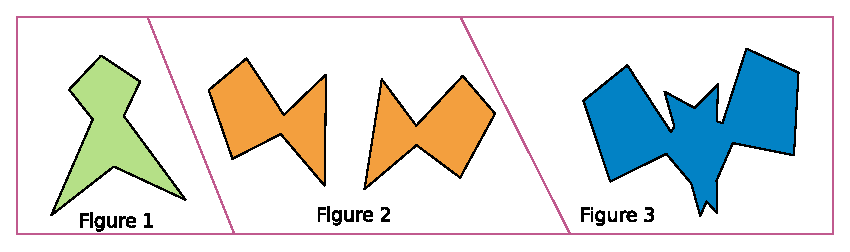
\includegraphics[width=14.5cm]{miroir} \end{center}

\begin{partie}
Observe les trois figures ci‑dessus :
\begin{enumerate}
 \item Quel est leur point commun ?
 
Comment peux‑tu le mettre en évidence ?
 \item Dans des publicités ou des magazines, trouve des images ou des logos qui ont la même propriété.
 \end{enumerate}
\end{partie}

\begin{minipage}[c]{0.54\linewidth}
\begin{partie}
À l'aide de papier calque, complète la figure ci‑contre avec un minimum de tracés pour que la droite d soit son \textbf{axe de symétrie}.
\end{partie}
\end{minipage}
\begin{minipage}[c]{0.44\linewidth}
\begin{center} 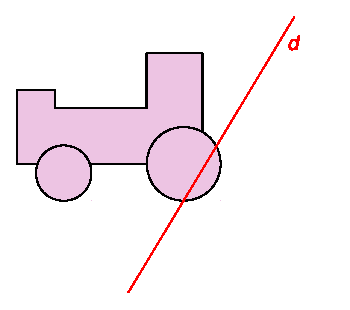
\includegraphics[width=4.5cm]{train} \end{center}
\end{minipage} \\

\end{activite}

%%%%%%%%%%%%%%%%%%%%%%%%%%%%%%%%%%%%%%%%%%%%%%%%%%%%%%%%%%%%%%%%%

\begin{activite}[Le symétrique dans l'œil]

\begin{center}
\begin{tabularx}{1.05\linewidth}{XXXX}
\begin{center} 
\includegraphics[width=3cm]{oeil1} \end{center} & \begin{center} 
\includegraphics[width=2.5cm]{oeil2} \end{center} & \begin{center} 
\includegraphics[width=3.2cm]{oeil3} \end{center} & \begin{center} 
\includegraphics[width=3.5cm]{oeil4} \end{center} \\
\begin{center} Figure 1 \end{center} & \begin{center} Figure 2 \end{center} & \begin{center} Figure 3 \end{center} & \begin{center} Figure 4 \end{center} \\
 \end{tabularx}
 \end{center}

\begin{partie} \label{SymAxCent_acti}
Observe les figures ci-dessus. La figure bleue est‑elle toujours symétrique à la figure orange par rapport à la droite tracée ? Justifie ta réponse en écrivant une phrase.
\end{partie}

\begin{partie}
Reproduis les figures ci‑dessous. Complète‑les à main levée en respectant la symétrie par rapport à la droite d et en tenant compte des remarques faites dans la partie \ref{SymAxCent_acti}.

\begin{minipage}[c]{0.48\linewidth}
\begin{center} 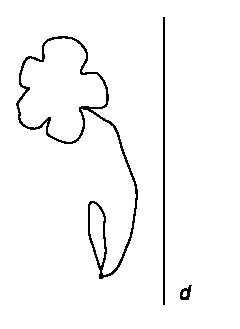
\includegraphics[width=3.5cm]{figure1} \end{center} 
 \end{minipage}
 \begin{minipage}[c]{0.48\linewidth}
 \begin{center} 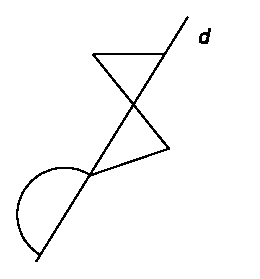
\includegraphics[width=3.5cm]{figure2} \end{center} 
  \end{minipage} \\
\end{partie}

\end{activite}

%%%%%%%%%%%%%%%%%%%%%%%%%%%%%%%%%%%%%%%%%%%%%%%%%%%%%%%%%%%%%%%%%

\begin{activite}[Une droite bien connue]

\begin{minipage}[c]{0.64\linewidth}
\begin{partie}
Sur la figure ci‑contre, quel est le symétrique du point $A$ par rapport à l'axe $d$ ? \\[0.5em]
Trouve les paires de points symétriques par rapport à la droite $d$. Décalque‑les ainsi que la droite $d$.
\end{partie}

\begin{partie}
Quel est le symétrique du point $J$ par rapport à l'axe $d$ ? Y a‑t‑il un autre point qui a la même particularité ?
\end{partie}

\begin{partie}
Sur ton calque, relie les points qui sont symétriques. Que peux-tu dire de la droite $d$ pour ces segments ?
\end{partie}
 \end{minipage}
  \qquad \begin{minipage}[c]{0.30\linewidth}
  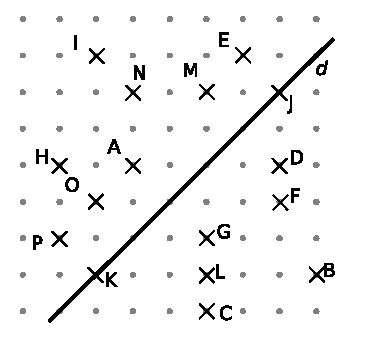
\includegraphics[width=5.5cm]{droite_connue}
  \end{minipage} \\
 

\begin{partie}
Trace le cercle de centre $J$ passant par $A$ et celui de centre $K$ passant par $A$. Que remarques‑tu ?
         
Trace un autre cercle passant par $A$ et $G$. Où doit se situer son centre ?
\end{partie}


\begin{partie}
Sur ton calque, place un point $T$ qui n'est pas sur la droite $d$. Propose deux façons de construire son symétrique $T'$ par rapport à $d$ sans plier le calque.
\end{partie}

\end{activite}

%%%%%%%%%%%%%%%%%%%%%%%%%%%%%%%%%%%%%%%%%%%%%%%%%%%%%%%%%%%%%%%%%

\begin{activite}[Un peu de mesure]

\begin{partie}[Symétrique d'un segment]
\begin{enumerate}
 \item Trace une droite $d$ et un segment $[AB]$. Construis le symétrique du segment $[AB]$ par rapport à la droite $d$.
 \item Compare les mesures des deux segments. Tes camarades obtiennent‑ils la même remarque ?
 
 \begin{minipage}[c]{0.52\linewidth}
 \item Romain avait construit le symétrique $A'B'C'$ du triangle $ABC$ par rapport à l'axe $d$. Malheureusement, sa feuille s'est déchirée et il ne reste que la figure ci‑contre. Romain doit déterminer le périmètre du triangle $ABC$. 
 
Explique comment il peut faire en utilisant uniquement la règle graduée et sans tracé supplémentaire.
  \end{minipage}
   \qquad \begin{minipage}[c]{0.46\linewidth}
  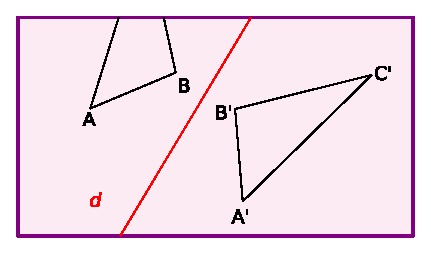
\includegraphics[width=5.5cm]{feuille_Romain}
  \end{minipage} \\
 \end{enumerate}
\end{partie}

\begin{partie}[Symétrique d'un cercle]
\begin{enumerate}
 \begin{minipage}[c]{0.62\linewidth}
 \item Reproduis la figure ci‑contre, place un point $M$ sur le cercle (\phantom{...}) puis construis les points $O'$ et $M'$ symétriques respectifs de $O$ et de $M$ par rapport à $d$.
 
Quelle est la longueur de $[O'M']$ ? Justifie ta réponse.
 \item Construis le symétrique du cercle (\phantom{...}) par rapport à la droite $d$.
  \end{minipage}
   \qquad \begin{minipage}[c]{0.36\linewidth}
  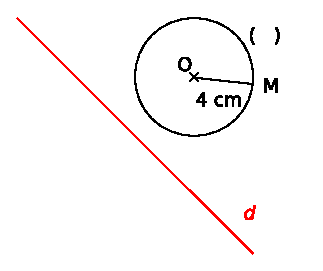
\includegraphics[width=4.5cm]{cercle_sym}
  \end{minipage} \\
 \end{enumerate}
\end{partie}

\end{activite}

%%%%%%%%%%%%%%%%%%%%%%%%%%%%%%%%%%%%%%%%%%%%%%%%%%%%%%%%%%%%%%%%%

\begin{activite}[Symétrique d'une droite]

\begin{minipage}[c]{0.62\linewidth}
\begin{partie}[Droite parallèle à l'axe]
\begin{enumerate}
 \item Trace deux droites parallèles \textcolor{B2}{$d$} et $d_1$ ;
 \item Construis la droite $d_2$ symétrique de la droite $d_1$ par rapport à l'axe \textcolor{B2}{$d$} ;
 \item Que peux‑tu dire des droites $d_1$ et $d_2$ ? Justifie ta réponse.
 \end{enumerate}
\end{partie}
 \end{minipage}
   \qquad \begin{minipage}[c]{0.36\linewidth}
  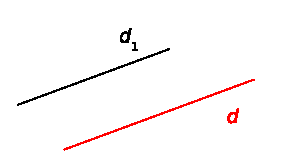
\includegraphics[width=4.5cm]{d1d}
  \end{minipage} \\

\vspace{1em}

\begin{minipage}[c]{0.62\linewidth}
\begin{partie}[Droite perpendiculaire à l'axe]
\begin{enumerate}
 \item Construis deux droites \textcolor{B2}{$d$} et $d_1$ perpendiculaires ;
 \item Place un point $A$ sur la droite $d_1$ et construis son symétrique $A'$ par rapport à l'axe \textcolor{B2}{$d$}. Justifie la position du point $A'$. \\[0.5em]
Que peux-tu dire alors de la droite $d_2$ symétrique de la droite $d_1$ par rapport à l'axe $d$ ?
 \end{enumerate}
\end{partie}
 \end{minipage}
   \qquad \begin{minipage}[c]{0.36\linewidth}
  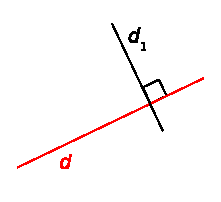
\includegraphics[width=3.5cm]{d1_perp_d}
  \end{minipage} \\

\end{activite}

%%%%%%%%%%%%%%%%%%%%%%%%%%%%%%%%%%%%%%%%%%%%%%%%%%%%%%%%%%%%%%%%%

%%%%%%%%%%%%%%%%%%%%%%%%%%%%%%%%%%%
%%%%%%%%%%%%%%%%%%%%%%%%%%%%%%%%%%%
%MiseEnPage
%%%%%%%%%%%%%%%%%%%%%%%%%%%%%%%%%%%
\newpage
%%%%%%%%%%%%%%%%%%%%%%%%%%%%%%%%%%%
%%%%%%%%%%%%%%%%%%%%%%%%%%%%%%%%%%%



\begin{activite}[Calque et demi-tour]

Mathieu a décalqué le bateau rose puis il l'a fait tourner autour du point $O$ dans le sens de la flèche. Il a dessiné quatre bateaux de couleurs différentes.

\vspace{1em}

\begin{minipage}[c]{0.52\linewidth}
\begin{partie}
Certains bateaux sont à moins d'un demi-tour, d'autres à plus d'un demi-tour du bateau de départ. Peux-tu préciser lesquels ?
\end{partie}

\begin{partie}
Reproduis, sur ton cahier, le bateau rose et le point $O$. À l'aide d'un morceau de papier calque, place un bateau qui soit à moins d'un demi-tour et un autre qui soit à plus d'un demi-tour du bateau de départ.
\end{partie}

\begin{partie} \label{SymAxCentActi2}
Mathieu remarque que lorsqu'il fait tourner le bateau rose autour du point $O$, le point $A$, tout en haut du mât, décrit une ligne qu'il connaît bien. Quelle est cette ligne ? Construis-la sur ton dessin.
\end{partie}
 \end{minipage}
   \quad \begin{minipage}[c]{0.26\linewidth}
  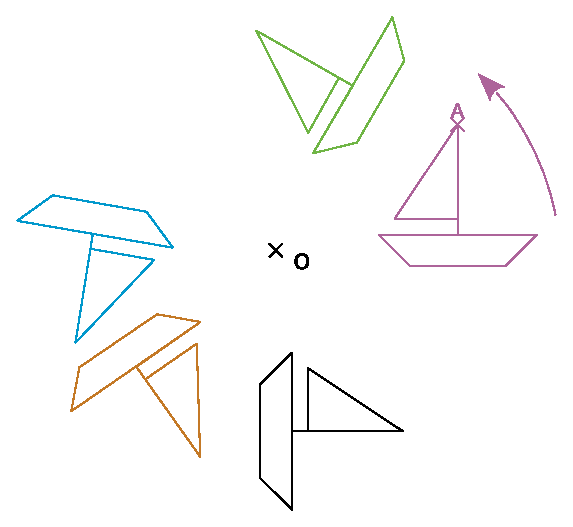
\includegraphics[width=6.7cm]{bateaux}
  \end{minipage} \\

\begin{partie} \label{SymAxCentActi3}
Mathieu aimerait bien construire un bateau qui soit exactement à un demi-tour du bateau rose. Pour savoir où s'arrêter de tourner, Mathieu se dit qu'il faudrait connaître la position exacte du point $A$ après un demi-tour. Construis ce point.
\begin{center} \textbf{\textcolor{H1}{Le demi-tour autour du point $O$ est encore appelé symétrie de centre $O$.}} \end{center}
\end{partie}

\begin{partie}
En t'aidant des parties \ref{SymAxCentActi2} et \ref{SymAxCentActi3}, construis le symétrique du bateau de départ par la symétrie de centre $O$.
\end{partie}

\end{activite}

%%%%%%%%%%%%%%%%%%%%%%%%%%%%%%%%%%%%%%%%%%%%%%%%%%%%%%%%%%%%%%%%%



\begin{activite}[Dans un quadrillage]

\begin{minipage}[c]{0.67\linewidth}
\begin{partie}
Reproduis la figure ci-contre sur ton cahier. \\[0.5em]
Pour aller de $O$ à $A$, on suit la flèche rose puis la verte.
\end{partie}
 \end{minipage}
  \qquad \begin{minipage}[c]{0.36\linewidth}
  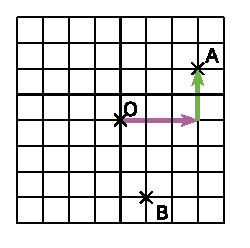
\includegraphics[width=3.7cm]{quadrillageAOB}
  \end{minipage} \\

\begin{partie}
En utilisant du papier calque, construis le symétrique de chaque flèche par rapport à $O$ puis complète les phrases suivantes : 
\begin{itemize}
 \item Le symétrique par rapport à un point d'une flèche de trois carreaux vers la droite est une flèche \ldots ;
 \item Le symétrique par rapport à un point d'une flèche de deux carreaux vers le haut est \ldots.
 \end{itemize}
\end{partie}
                
\begin{partie}
À l'aide des symétriques des flèches rose et verte, place le point $A'$, symétrique du point $A$ par rapport à $O$.
\end{partie}
         
\begin{partie}
En utilisant uniquement le quadrillage et en t'inspirant de la méthode découverte ci-dessus, place le point $B'$ symétrique du point $B$ par rapport à $O$.
\end{partie}

\end{activite}

%%%%%%%%%%%%%%%%%%%%%%%%%%%%%%%%%%%%%%%%%%%%%%%%%%%%%%%%%%%%%%%%%

\begin{activite}[Centre de symétrie]

\begin{partie}
Construis un segment $[RS]$ de 5 cm de longueur. Quel est son centre de symétrie ?
\end{partie}


\begin{partie}
Construis un cercle de centre $O$ et de rayon 3 cm. Quel est son centre de symétrie ?
\end{partie}
         
         
\begin{partie}
Construis une droite $d$. Combien admet-elle de centres de symétrie ?
\end{partie}
         
         
\begin{partie}
Est-il possible de construire un triangle non aplati qui a un centre de symétrie ?
\end{partie}
         
         
\begin{partie}
Place trois points non alignés $A$, $B$ et $O$. Construis les points $C$ et $D$ pour que le quadrilatère $ABCD$ ait le point $O$ comme centre de symétrie.
\end{partie}
        
\vspace{1em}

\begin{minipage}[c]{0.62\linewidth}
\begin{partie}
Sur ton cahier, place trois points $Z$, $V$ et $W$ comme sur la figure ci-contre. Comment construire le point $M$ pour que le quadrilatère $ZVWM$ ait un centre de symétrie ?
\end{partie}         
              
         
\begin{partie}
Construis un hexagone $EFGHIJ$ qui admet un centre de symétrie.
\end{partie}
 \end{minipage}
  \qquad \begin{minipage}[c]{0.36\linewidth}
  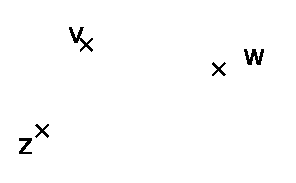
\includegraphics[width=4.5cm]{pointsVWZ}
  \end{minipage} \\

\end{activite}

%%%%%%%%%%%%%%%%%%%%%%%%%%%%%%%%%%%%%%%%%%%%%%%%%%%%%%%%%%%%%%%%%
